\chapter{Introducción específica} % Main chapter title

\label{Chapter2}

%----------------------------------------------------------------------------------------
%	SECTION 1
%----------------------------------------------------------------------------------------
Esta sección presenta los requerimientos acordados con el cliente, las diferentes tecnologías a utilizar y las herramientas y recursos utilizados para realizar el trabajo.

\section{Requerimientos acordados con el cliente}
\subsection{Requerimientos funcionales:}
	\begin{itemize}
		\item \textbf{Requerimientos de \textit{hardware}:}
			\begin{enumerate}
				\item El dispositivo deberá contar con un transformador de 110 / 220 VAC a 24 VAC a 2 A que será utilizado para alimentar el microcontrolador, sensores y periféricos de entrada y salida.
				\item El dispositivo deberá contar con un rectificador y regulador de tensión a 5 VDC y 3.3 VDC.
				\item El dispositivo deberá contar con una interface USB para su programación, actualización de código y depuración.
				\item El dispositivo deberá contar con una pantalla LCD o similar de mínimo 2.4'' hasta 3.5''.
				\item El dispositivo deberá contar con un \textit{joystick} o botoneras para su manipulación y configuración.
				\item El dispositivo deberá contar con un \textit{Real Time Clock} (RTC), el mismo que deberá mantener la fecha y hora actual ante un corte de energía.
				\item El dispositivo deberá contar con un sensor de temperatura que mida mínimo en el rango de -20 °C a 60 °C con una precisión de +/- 1 °C o inferior.
				\item El dispositivo deberá contar con un sensor de humedad relativa de 0-100 \% con una precisión de +/- 3 \% o inferior.
				\item El dispositivo deberá contar con un sensor de presión atmosférica que mida en el rango de 300 a 1100 hPa (0.3 - 1.1 bar) con una precisión absoluta de +/- 1 hPa o inferior.
				\item El dispositivo deberá contar con cuatro (4) salidas independientes para las electroválvulas de 24 VAC y las mismas que deberán ser energizadas por el propio transformador del dispositivo.
				\item El dispositivo deberá contar con una (1) salida independiente para la motobomba.
				\item El dispositivo deberá soportar la tecnología Wi-Fi para envío y recepción de datos.	
			\end{enumerate}
			
		\item \textbf{Requerimientos de \textit{firmware}:}
			\begin{enumerate}	
				\item Se deberá usar el idioma español o ingles.
				\item La pantalla LCD debe mostrar el menú de opciones de configuración:
					\begin{itemize}
						\item Establecer fecha y hora
						\item Programar secuencias de riego
						\item Riego manual
						\item Activar/Desactivar válvulas
					\end{itemize}
				\item Se debe permitir establecer la fecha y hora a través del \textit{joystick} o botoneras, el formato a utilizar será de 24 hrs.
				\item Se debe permitir programar las secuencias de riego de cada electroválvula de manera independiente siguiendo las siguientes consideraciones:
					\begin{itemize}
						\item Configurar la hora de ejecución de riego en horas, minutos y segundos.
						\item Configurar la duración de riego en horas, minutos y segundos.
						\item Configurar la frecuencia expresado en horas y minutos. Por ejemplo, ejecutar el riego cada 2 horas.
						\item Seleccionar los días de riego.
						\item Poder borrar la configuración actual de la secuencia de riego.
					\end{itemize}		
				\item Se debe permitir encender cada electroválvula de manera manual independientemente de la programación que tenga configurada.
				\item Se debe permitir activar y desactivar cada secuencia de riego de manera independiente.
				\item La pantalla LCD debe mostrar un \textit{dashboard} con la siguiente información:
					\begin{itemize}
						\item La fecha y hora actual.
						\item La programación actual de las secuencias de riego.
						\item La presión atmosférica (altitud).
						\item La temperatura y humedad ambiental.
						\item El estado de los sensores de nivel de agua de los tanques.
						\item El estado de las electroválvulas (encendidas/apagadas).
					\end{itemize}
			\end{enumerate}
	\end{itemize}

\subsection{Requerimientos no funcionales:}
	\begin{enumerate}
		\item El tiempo de muestreo de los sensores de temperatura, humedad y presión atmosférica será de 5 segundos como máximo.
		\item Se debe garantizar un soporte post venta de 5 años.
	\end{enumerate}

\subsection{Historias de usuario}
\label{sec:backlog}
Para la ponderación de la dificultad, complejidad e incertidumbre de las historias de usuarios se usará la serie de Fibonacci y se clasificará en tres niveles: 
\begin{itemize}
\item Baja (1)
\item Media (3)
\item Alta (5).
\end{itemize}

El puntaje total será redondeado hacia arriba al valor mas cercano de la serie de Fibonacci. Por ejemplo, si la sumatoria da como resultado 11, el Story Point a considerar será 13.

\textbf{Historia 1:}
''Como operario, quiero que el idioma del dispositivo sea español por un tema de facilidad de uso''.
\begin{itemize}
\item \textbf{Dificultad:} baja (1)
\item \textbf{Complejidad:} baja (1)
\item \textbf{Incertidunbre:} baja (1)
\newline
\newline
\textbf{\textit{Story Point}: 3}
\end{itemize}

\textbf{Historia 2:}
''Como agricultor, quiero poder visualizar el día, mes, año, hora, minuto, temperatura, humedad y presión atmosférica (altitud) en tamaño visible''.
\begin{itemize}
\item \textbf{Dificultad:} alta (5)
\item \textbf{Complejidad:} media (3)
\item \textbf{Incertidunbre:} media (3)
\newline
\newline
\textbf{\textit{Story Point:} 13}
\end{itemize}

\textbf{Historia 3:}
''Como agricultor, quiero tener la posibilidad de programar los riegos una vez al día o varias veces al día, un vez a la semana o varios días a la semana''.
\begin{itemize}
\item \textbf{Dificultad:} alta (5)
\item \textbf{Complejidad:} alta (5)
\item \textbf{Incertidunbre:} media (3)
\newline
\newline
\textbf{\textit{Story Point:} 13}
\end{itemize}

\textbf{Historia 4:}
''Como operario, quiero que en caso sea necesario usar una motobomba, esta última se active después de haberse iniciado la secuencia de riego''.
\begin{itemize}
\item \textbf{Dificultad:} media (3)
\item \textbf{Complejidad:} baja (1)
\item \textbf{Incertidunbre:} baja (1)
\newline
\newline
\textbf{\textit{Story Point:} 5}
\end{itemize}

\textbf{Historia 5:}
''Como operario, quiero que cuando haya transcurrido el tiempo de riego, primero se apague la motobomba y después se cierren las electroválvulas para evitar daños en la motobomba''.
\begin{itemize}
\item \textbf{Dificultad:} media (3)
\item \textbf{Complejidad:} baja (1)
\item \textbf{Incertidunbre:} baja (1)
\newline
\newline
\textbf{\textit{Story Point:} 5}
\end{itemize}

\textbf{Historia 6:}
''Como agricultor, quiero que el dispositivo tenga la capacidad de controlar una motobomba para darle mayor presión al agua en caso sea necesario.
\begin{itemize}
\item \textbf{Dificultad:} baja (1)
\item \textbf{Complejidad:} baja (1) 
\item \textbf{Incertidunbre:} baja (1) 
\newline
\newline
\textbf{\textit{Story Point:} 3}
\end{itemize}

\textbf{Historia 7:}
''Como agricultor, quisiera que el dispositivo incluya sus propias electroválvulas para evitarme el trabajo de buscar esas partes fuera y/o tener problemas de incompatibilidad.
\begin{itemize}
\item \textbf{Dificultad:} baja (1)
\item \textbf{Complejidad:} baja (1)
\item \textbf{Incertidunbre:} baja (1)
\newline
\newline
\textbf{\textit{Story Point:} 3}
\end{itemize}

\textbf{Historia 8:}
''Como operario, quisiera poder activar de forma voluntaria las electroválvulas e iniciar una secuencia de riego manual sin depender y desconfigurar la secuencia de riego programada.
\begin{itemize}
\item \textbf{Dificultad:} media (3)
\item \textbf{Complejidad:} media (3)
\item \textbf{Incertidunbre:} baja (1)
\newline
\newline
\textbf{\textit{Story Point:} 8}
\end{itemize}

\textbf{Historia 9:}
''Como agricultor, quisiera poder deshabilitar la secuencia de riego de manera temporal sin borrar la configuración ya establecida. Esto sería útil cuando se tenga que realizar algún mantenimiento en las cañerías o durante las temporadas de cosecha.
\begin{itemize}
\item \textbf{Dificultad:} baja (1) 
\item \textbf{Complejidad:} media (3) 
\item \textbf{Incertidunbre:} baja (1) 
\newline
\newline
\textbf{\textit{Story Point:} 5}
\end{itemize}

\section{Tecnologías utilizadas}
\subsection{ESP32:}
Como cerebro del dispositivo se utilizó el \textit{System on a Chip} ESP32 del fabricante Espressif. El ESP32 emplea un microprocesador Tensilica Xtensa LX6 de doble núcleo.

\begin{figure}[h]
	\centering
	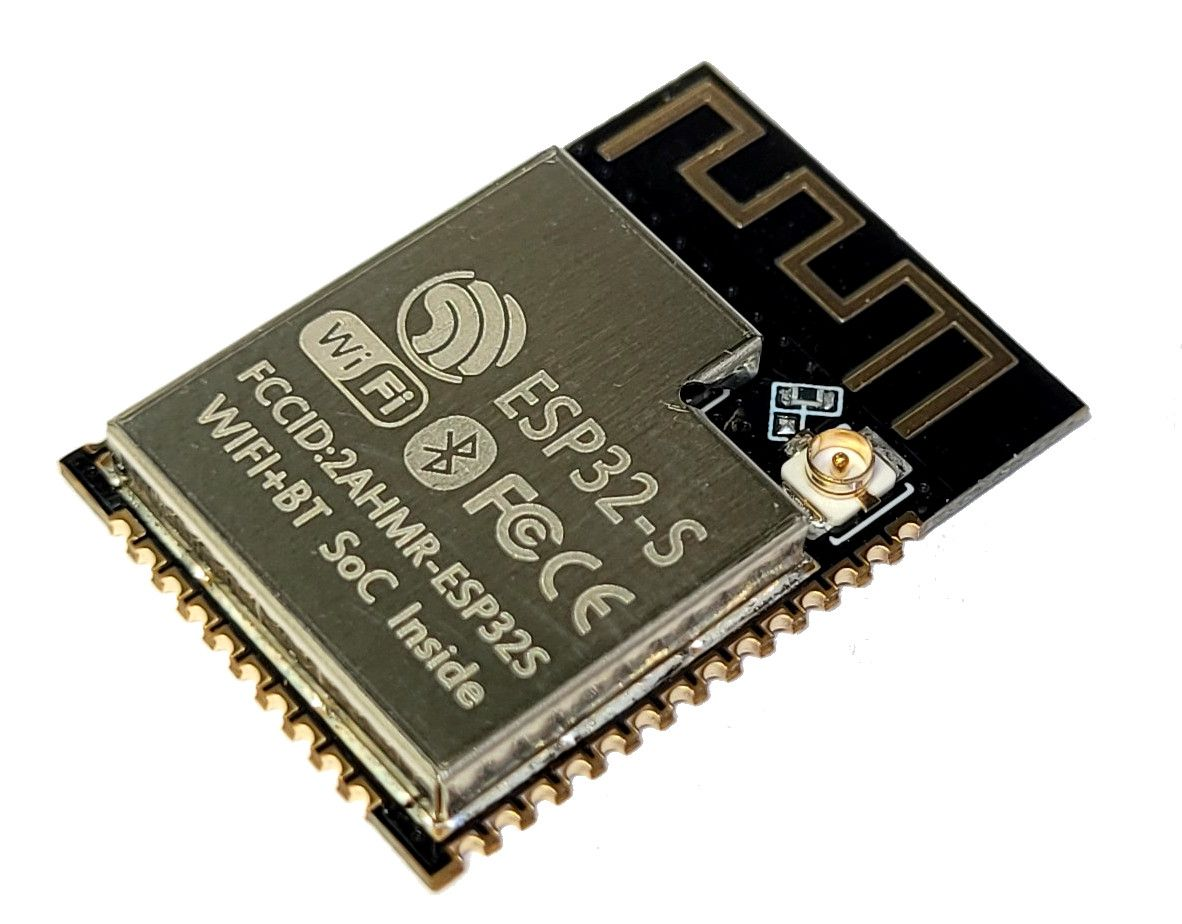
\includegraphics[width=0.4\textwidth]{SoC ESP32}
	\caption{System on a Chip Espressif ESP32}
\end{figure}

Entre las principales características del ESP32 son:
\begin{enumerate}
	\item Procesador:
	\begin{enumerate}
		\item CPU: microprocesador de 32-bit Xtensa LX6 de doble núcleo (o de un solo núcleo), operando a 160 o 240 MHz y rindiendo hasta 600 DMIPS.
		\item Co-procesador de ultra baja energía (ULP).
	\end{enumerate}
	\item Memoria: 520 KiB SRAM.
	\item Conectividad inalámbrica:
	\begin{enumerate}
		\item Wi-Fi: 802.11 b/g/n.
		\item Bluetooth: v4.2 BR/EDR y BLE.
	\end{enumerate}
	\item Periféricos:
	\begin{enumerate}
		\item 12-bit SAR ADC de hasta 18 canales.
		\item 2 × 8-bit DACs.
		\item 10 × sensores de tacto (sensores capacitivos GPIOs).
		\item 4 × SPI.
		\item 2 × interfaces I²S.
		\item 2 × interfaces I²C.
		\item 3 × UART
		\item Controlador host SD/SDIO/CE-ATA/MMC/eMMC
		\item Controlador esclavo SDIO/SPI
		\item Interfaz Ethernet MAC con DMA dedicado y soporte para el protocolo IEEE 1588 Precision Time Protocol.
		\item Bus CAN 2.0.
		\item Controlador remoto infrarrojo (TX/RX, hasta 8 canales).
		\item Motor PWM.
		\item LED PWM (hasta 16 canales).
		\item Sensor de efecto Hall
		\item Pre-amplificador analógico de ultra baja potencia
	\end{enumerate}
	\item Seguridad:
	\begin{enumerate}
		\item Soporta todas las características de seguridad estándar de IEEE 802.11, incluyendo WFA, WPA/WPA2 y WAPI.
		\item Arranque seguro.
		\item Cifrado flash.
		\item 1024-bit OTP, hasta 768-bit para clientes.
		\item Criptografía acelerada por hardware: AES, SHA-2, RSA, criptografía de curva elíptica (ECC), generador de números aleatorios (RNG).
	\end{enumerate}	
\end{enumerate}



\subsection{Pantalla TFT de 3.5 pulgadas:}

\subsection{Joystick:}

\subsection{Sensor BME280:}

\subsection{Chip FT232RL:}

\section{Herramientas y recursos de terceros}

